\newpage
\section*{Problem 4:}

Figure \ref{fig:problem_4} shows the associated graph $G(A)$ of matrix $A$ along with the steps of the minimum degree algorithm. From these steps, the reordering of the nodes will be $[2,\ 4,\ 5,\ 3,\ 6,\ 7,\ 1,\ 8, \9]$



\begin{figure}[!tbh]
\centering        
   \subfloat{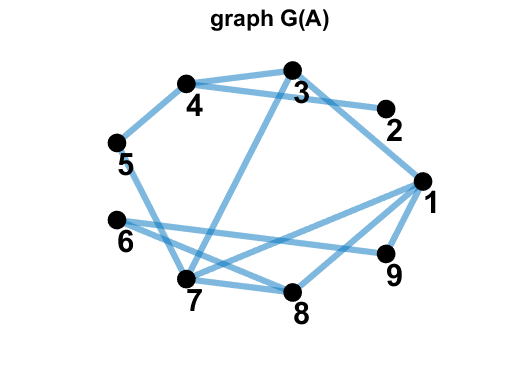
\includegraphics[width=0.33\textwidth]{../code/0.png}}
   \subfloat{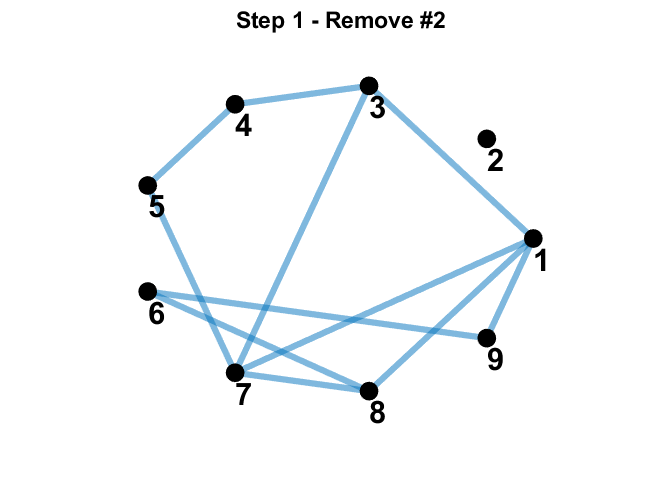
\includegraphics[width=0.33\textwidth]{../code/1.png}}   
   \subfloat{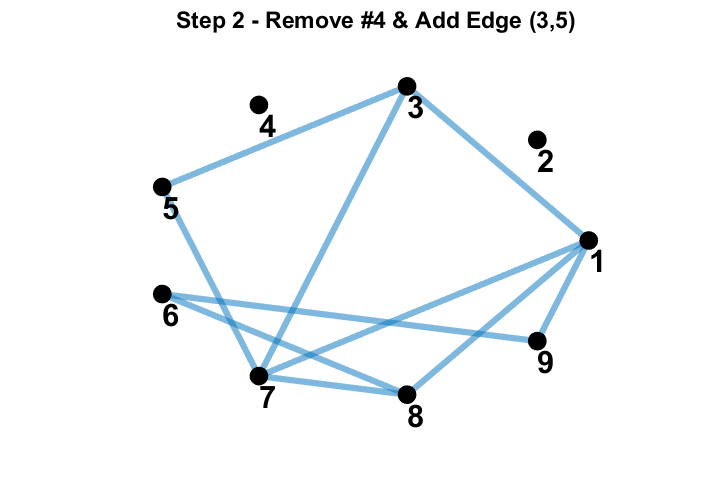
\includegraphics[width=0.33\textwidth]{../code/2.png}}
    
   \subfloat{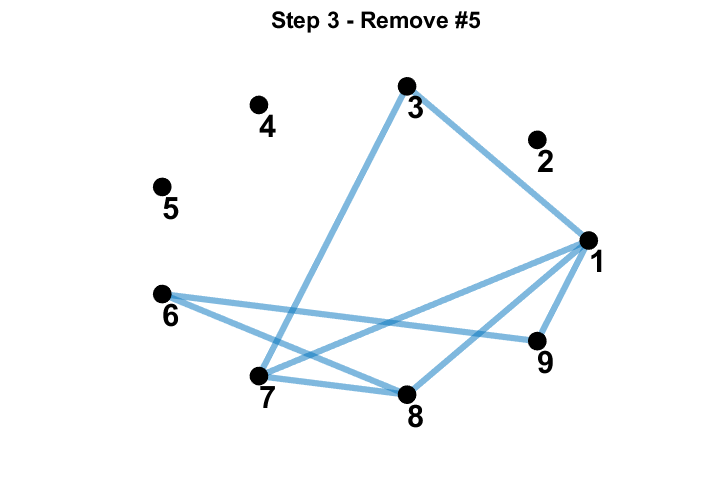
\includegraphics[width=0.33\textwidth]{../code/3.png}}
   \subfloat{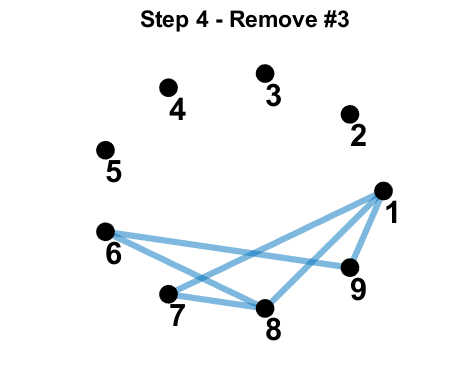
\includegraphics[width=0.33\textwidth]{../code/4.png}}
   \subfloat{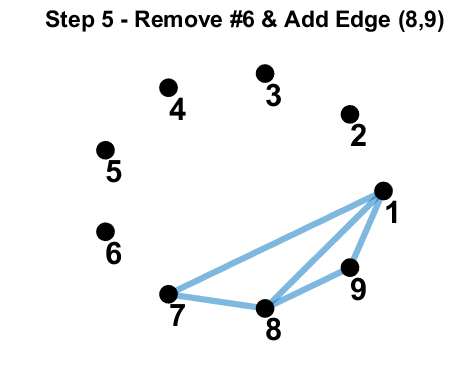
\includegraphics[width=0.33\textwidth]{../code/5.png}}
   
   \subfloat{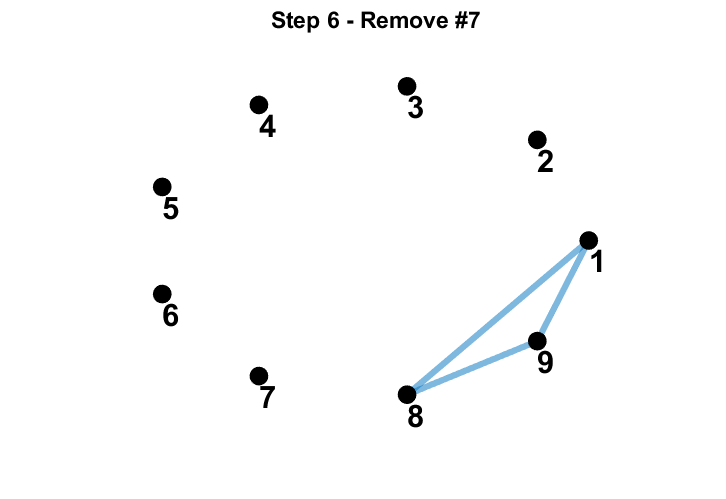
\includegraphics[width=0.33\textwidth]{../code/6.png}}
   \subfloat{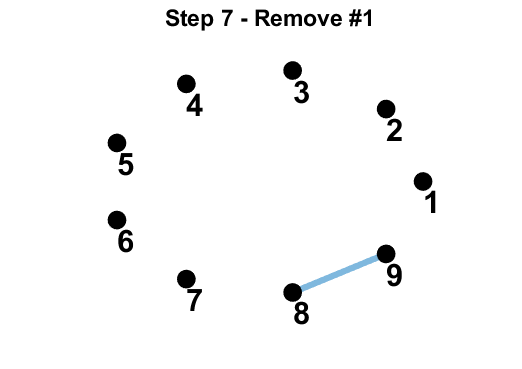
\includegraphics[width=0.33\textwidth]{../code/7.png}}
   \subfloat{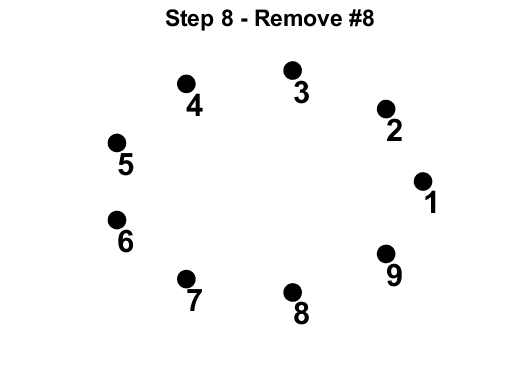
\includegraphics[width=0.33\textwidth]{../code/8.png}}
   \caption{Graph $G(A)$ along with the 8 steps of the minimum degree algorithm applied on it. }
   \label{fig:problem_4}
\end{figure}
